\documentclass[a4paper]{article}    % base article class
\usepackage[utf8]{inputenc}         % allow utf8 input
\usepackage{textalpha}              % enable greek utf8 in text
\usepackage{alphabeta}              % enable greek utf8 in math
\usepackage{graphicx}               % includegraphics
\usepackage{amsmath,amsthm}         % fancier math
%
%\usepackage{ebgaramond}
%
%\usepackage{newtxtext}               % times new roman font
%\usepackage[bigdelims,cmintegrals,vvarbb]{newtxmath}
%
\usepackage[osf,sups]{Baskervaldx} % lining figures
\usepackage[bigdelims,cmintegrals,vvarbb,baskervaldx,frenchmath,upint]{newtxmath} % math font
%\usepackage{cabin}                  % monospace font
\usepackage[cal=boondoxo]{mathalfa} % mathcal from STIX, unslanted a bit
%
\usepackage{hyperref,url}           % hyperlinks and urls
\usepackage{fancyvrb}               % fancier verbatim environment
\usepackage[x11names]{xcolor}                 % for colors
%\usepackage{pdflscape}              % for landscape pages
%\delimitershortfall-1sp
%\usepackage{mleftright}              % enlarge nested parentheses
%\mleftright
\setlength{\parindent}{0pt}         % no paragraph indentation
\setlength{\parskip}{7pt}           % spacing between paragraphs
\setlength{\emergencystretch}{3em}  % prevent overfull lines
\pdfimageresolution 200             % change the default for included png files
\pdfinfoomitdate=1\pdftrailerid{}   % ensure reproducible PDF
\makeatletter\renewcommand{\verbatim@font}{\ttfamily\footnotesize}\makeatother
\newenvironment{gallery}{}{}
\newcommand{\galleryline}[1]{\includegraphics{#1}{\footnotesize\tt #1}\newline}
\theoremstyle{note}
\newtheorem{exercice}{Exercice}
\swapnumbers
\theoremstyle{plain}
\newtheorem{theorem}{Theorem}[section]
\newtheorem{lemma}[theorem]{Lemma}
\newtheorem{remark}[theorem]{Remark}
\newtheorem{definition}[theorem]{Definition}
\newtheorem{proposition}[theorem]{Proposition}

\begin{document}

\title{tropomi pixel gain correction}
\date{}
\maketitle


\section{Introduction}

If you work with TROPOMI products you'll certainly recognize these
characteristic diagonal streaks

\begin{tabular}{ll}
	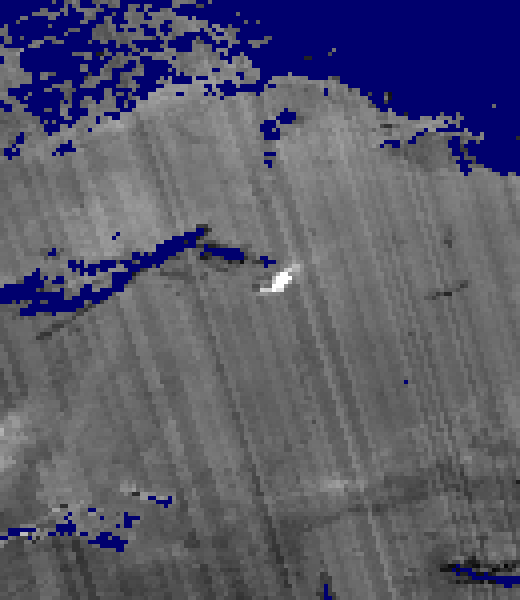
\includegraphics[width=.4\textwidth]{f/kccplume20b.png} &
	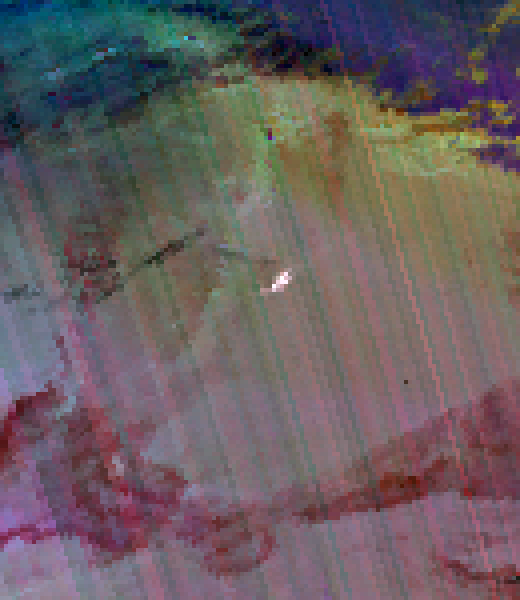
\includegraphics[width=.4\textwidth]{f/ikniceshot.png} \\
%	L2 product & Heuristic from L1
\end{tabular}

These streaks only seem to be diagonal because you are resampling the image on a
(longitude, latitude) grid.  In the raw image, which is acquired from a
slightly oblique orbit, they are aligned with the pixel grid


% plambda TRANS[flip=topdown,y=880,h=240]:S5P_OFFL_L2__CH4____20200105T112716_20200105T130846_11550_01_010302_20200107T042409.nc,methane_mixing_ratio_bias_corrected  'x 1e30 > nan x if'|qeasy 1830 1940|plambda 'x x 0 0 110 rgb if'|homwarp -o 0 -i "2 0 0 0 1 0 0 0 1" 430 240 |ntiply 4 - ~/cropblue.png
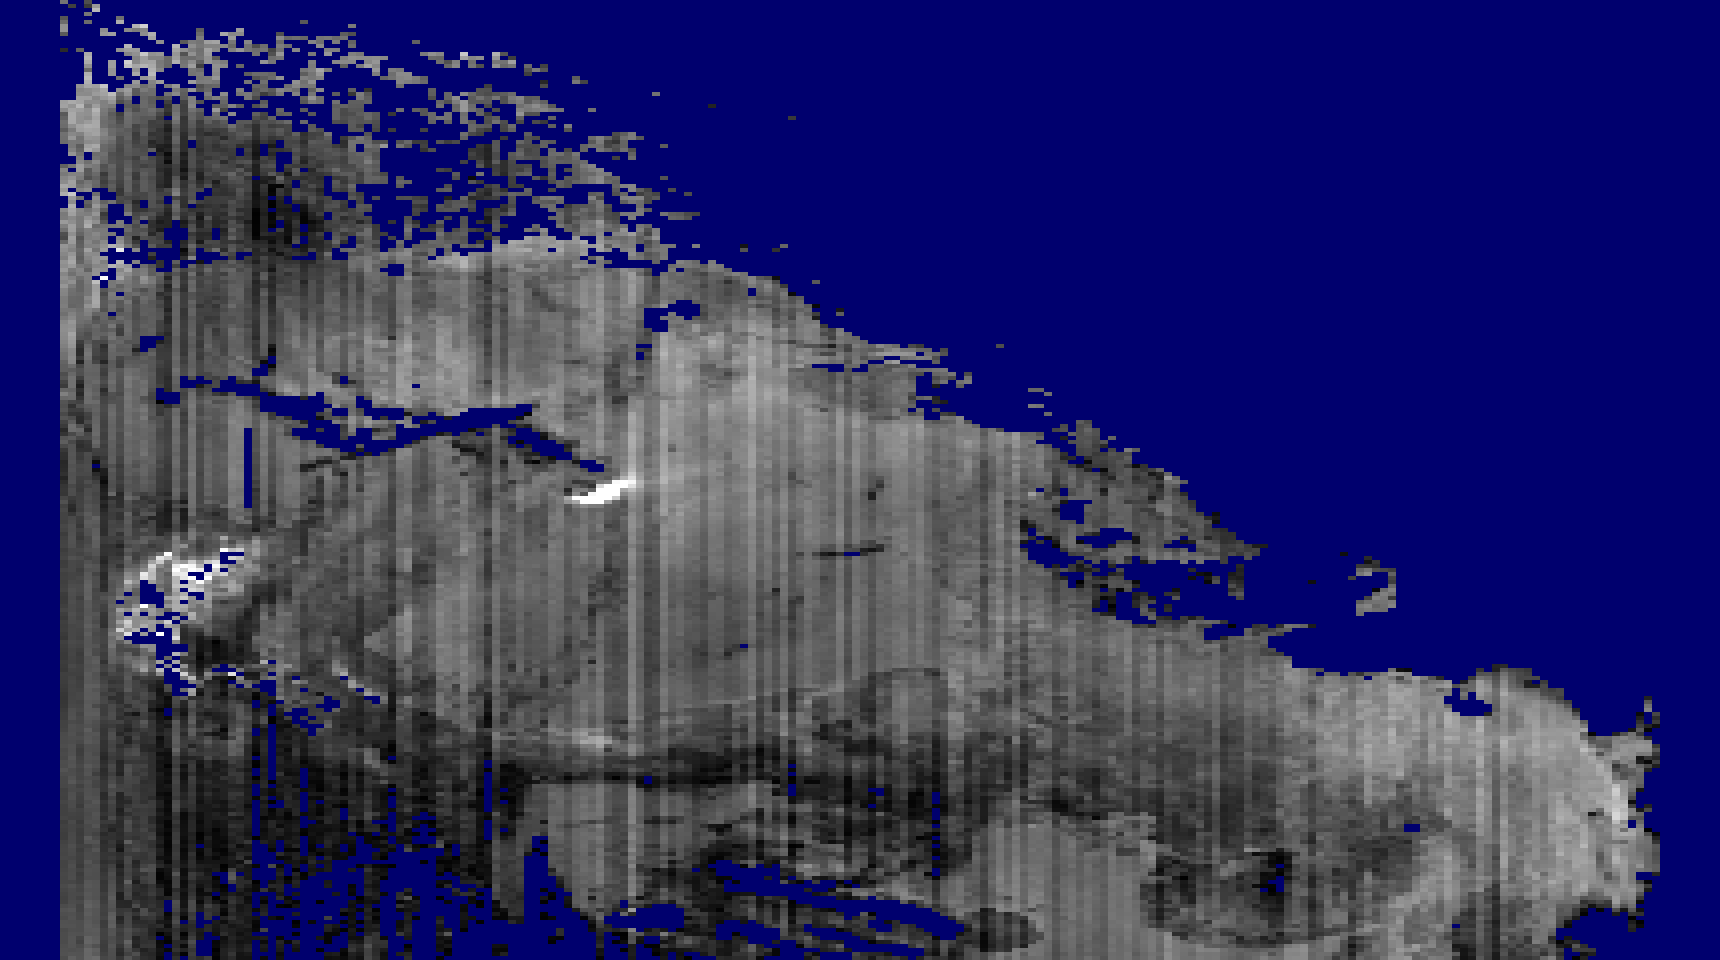
\includegraphics[width=.8\textwidth]{f/cropblue.png}

The objective of this note is to understand the origin of these artifacts and
propose two methods to remove them.

\section{Formation of the artifacts in the sensor}

The TROPOMI instruments contains four spectrometers: UV, UVIS, NIR and SWIR.
For archival purposes, the data of each of the detectors is divided in two
halves, which yields a total of eight spectral bands.  The UV, UVIS and NIR
detectors are three identical CCD matrices of size~$1024\times 1024$, of
which only about~$864$ rows are illuminated by the signal.  The SWIR detector
is a MCT ROIC matrix of size~$1000\times 256$.

The following 

\begin{tabular}{ll}
	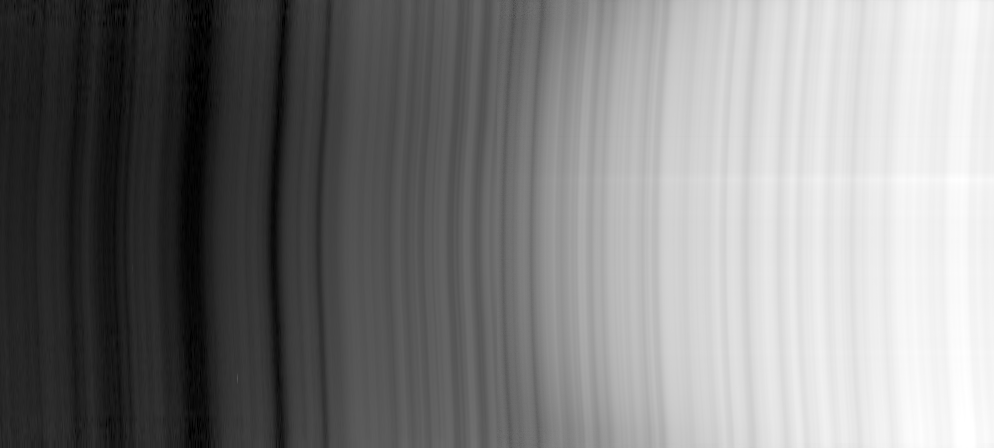
\includegraphics[width=0.48\linewidth]{f/lglint_12.png} &
	
\includegraphics[width=0.48\linewidth]{f/lglint_34.png} \\
	UV (bands 1 and 2)& UVIS (bands 3 and 4) \\
	& \\
	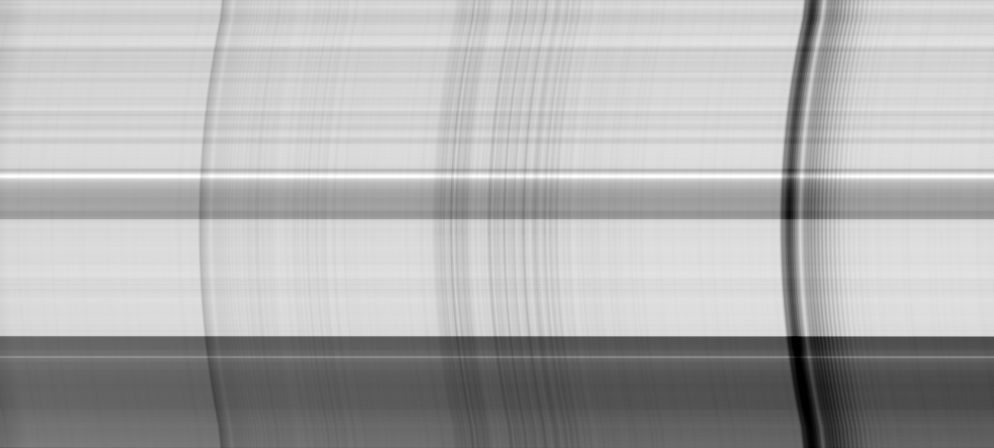
\includegraphics[width=0.48\linewidth]{f/lglint_56.png} &
	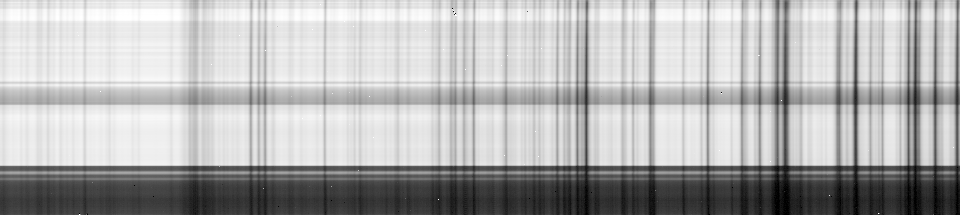
\includegraphics[width=0.48\linewidth]{f/lglint_78.png} \\
	NIR (bands 5 and 6) & SWIR (bands 7 and 8)
\end{tabular}


\begin{tabular}{l}
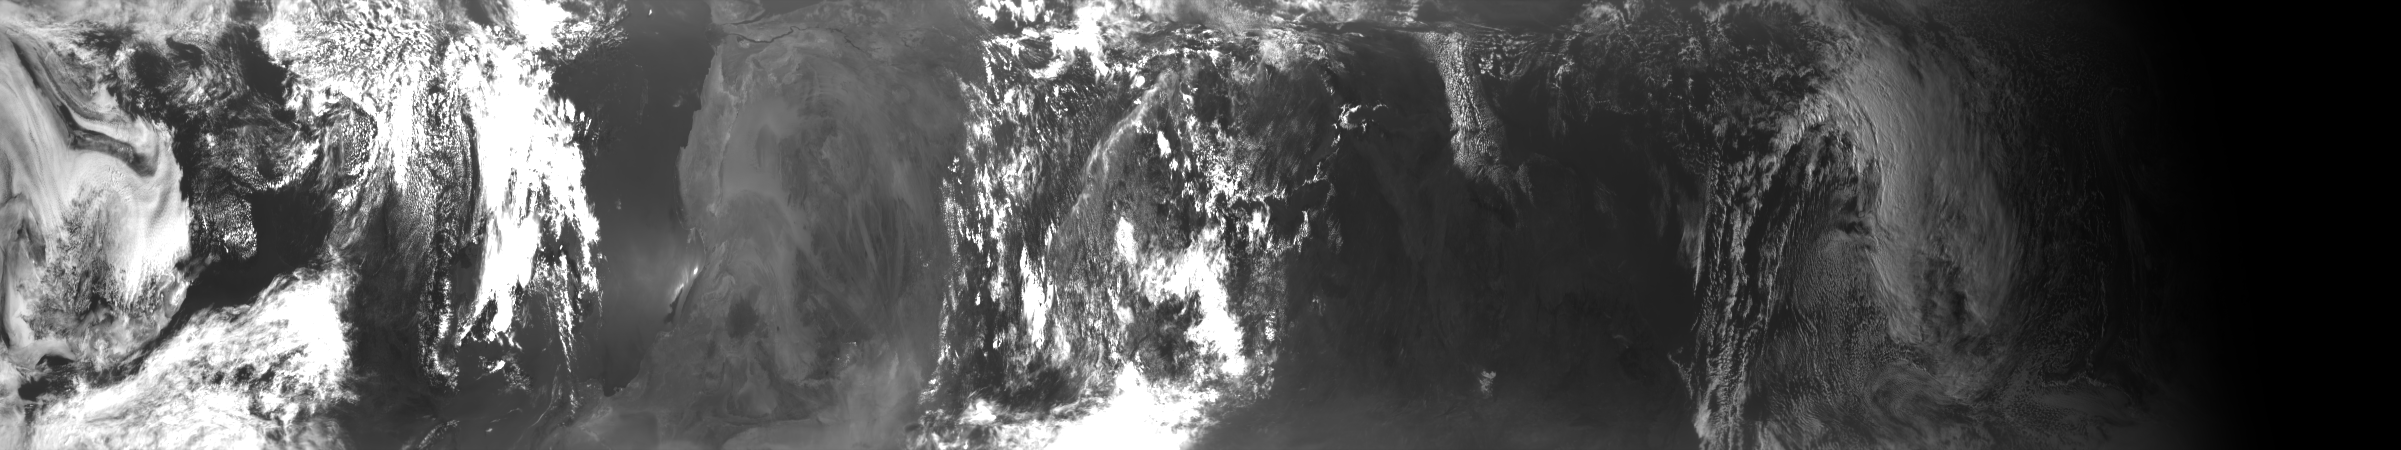
\includegraphics[width=\linewidth]{f/slice_b4_glint.png} \\
Average of all channels on band 4
\end{tabular}


There are two sources of anomalous readings: biases in the gain of each pixel
(which are not constant but vary slowly in time) and transient pixels due to
cosmic rays hitting the sensor array.  The gain of each pixel is typically
correlated along columns of the array, giving a characteristic texture
similar to that of the infrared cameras, that can be corrected by standard
means.  The transient pixels are isolated in space and frequency and can be
removed due to the local smoothness of the data.


\section{Method 1: data-based correction}

\section{Method 2: irradiance-based correction}


\end{document}


% vim:set tw=77 filetype=tex spell spelllang=en ts=2 sw=2:
